\documentclass[aps,pre,onecolumn,superscriptaddress,floatfix,nofootinbib]{revtex4-2}

\usepackage{amsmath,amssymb}
\usepackage{graphicx}
\usepackage{placeins}
\usepackage[colorlinks=true,allcolors=blue]{hyperref}


% --- Convencion de APS para Supplemental Material -------------------------
% El SM se publica como documento SEPARADO, asi que su numeracion no puede
% colisionar con la del manuscrito. Sin esto, [1] es Daubechies aqui y
% Levitov-Lesovik alla, y FIG. 1 y TABLE I significan cosas distintas en cada
% fichero. Se prefija todo con S: referencias, figuras, tablas y ecuaciones.
% La bibliografia es PROPIA -el SM debe ser autocontenido- y comparte refs.bib
% con el manuscrito para que una entrada no se edite en un sitio y no en el otro.
\renewcommand{\citenumfont}[1]{S#1}
\renewcommand{\bibnumfmt}[1]{[S#1]}
\renewcommand{\thefigure}{S\arabic{figure}}
\renewcommand{\thetable}{S\arabic{table}}
\renewcommand{\theequation}{S\arabic{equation}}

\newcommand{\avg}[1]{\left\langle #1 \right\rangle}
\newcommand{\Var}{\mathrm{Var}}
\newcommand{\eps}{\varepsilon}
\newcommand{\dd}{\mathrm{d}}

\begin{document}

\title{Supplemental Material for ``Temporal Organization Amplifies Counting
Fluctuations in Signed Order Flow''}

\author{Nelson Bol\'{\i}var}
\affiliation{Escuela de F\'isica, Facultad de Ciencias, Universidad Central de Venezuela, Caracas 1041-A, Venezuela}
\affiliation{Astrum Drive Technologies, 13024 Dallas Pkwy Unit 120 B, Frisco, TX 75034, USA}
\author{Gabriel Abell\'an}
\affiliation{Escuela de F\'isica, Facultad de Ciencias, Universidad Central de Venezuela, Caracas 1041-A, Venezuela}
\affiliation{Astrum Drive Technologies, 13024 Dallas Pkwy Unit 120 B, Frisco, TX 75034, USA}
\author{David Verrilli}
\affiliation{Escuela de F\'isica, Facultad de Ciencias, Universidad Central de Venezuela, Caracas 1041-A, Venezuela}

\maketitle

\section{Higher cumulants do not define a Gaussian crossover}

For each asset and dyadic counting window $T=1,2,4,\ldots,128$ hours, we form
non-overlapping accumulated flows $Q_T$ and report the standardised third and
fourth cumulants
\begin{equation}
 \gamma_1(T)=\frac{\kappa_3(T)}{\kappa_2(T)^{3/2}},\qquad
 \gamma_2(T)=\frac{\kappa_4(T)}{\kappa_2(T)^2}.
\end{equation}
The $95\%$ intervals use $999$ circular moving-block bootstrap replicates. The
block length corresponds to four weeks of clock time at every $T$, so the
resampling retains short- and intermediate-range dependence within each block.

Neither statistic approaches zero uniformly across assets
[Fig.~\ref{fig:supp-cumulants} and Table~\ref{tab:supp-cumulants}]. BTC loses
most of its excess kurtosis by $T=128$ but remains skewed; ETH becomes markedly
more skewed and heavy-tailed; BNB and SOL retain nonzero excess kurtosis. We
therefore do not define a characteristic Gaussian scale $T^*$. This does not
alter the algebraic statement in the main text: Gaussianity is a sufficient null
explanation for a linear symmetry function, not an empirical description we
impose on all windows. Conversely, a linear $\log[P(Q)/P(-Q)]$ can occur for a
non-Gaussian exponentially tilted distribution, so linearity alone does not
establish either Gaussianity or a nontrivial fluctuation theorem.

\begin{figure}[t]
 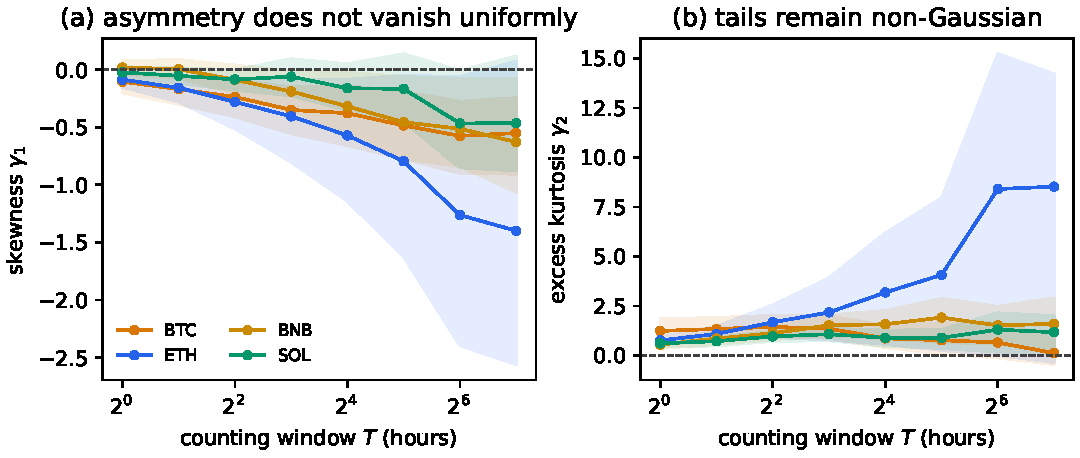
\includegraphics[width=\linewidth]{../output/figuras/fig13_standardized_cumulants.pdf}
 \caption{Scale dependence of (a) skewness and (b) excess kurtosis for the
 hourly BTC, ETH, BNB, and SOL series. Shading is the moving-block bootstrap
 $95\%$ interval. The zero line is the Gaussian value.}
 \label{fig:supp-cumulants}
\end{figure}

\subsection*{Cubic fits to the symmetry function}

The Gaussian identity predicts $s(Q)$ exactly linear in $Q$. We therefore fit
$s(Q)=A\,Q+c_3\,Q^3$ and ask whether $c_3$ is resolved. Linearity is consistent
with the data in BNB and SOL at every window and both resolutions, with
$|c_3|/\sigma_{c_3}\le1.3$. ETH is marginal at $T=1$ ($-2.1\sigma$ hourly) and
consistent with zero at all larger windows ($0.2\sigma$ at $T=16$, hourly). BTC
is the exception: $c_3/\sigma_{c_3}=3.9$ hourly and $4.5$ four-hourly at $T=1$,
falling to $2.2$ and $1.5$ by $T=16$. The reduced $\chi^2$ of the BTC fits
ranges $1.3$--$3.4$ across dyadic windows and both resolutions, never near
unity, so the parametric form is in any case a poor description there.

This is the expected pattern rather than a difficulty. Gaussianity implies
exact linearity of $s(Q)$, but linearity does not imply Gaussianity: a
non-Gaussian exponentially tilted symmetric distribution can have the same
property. Conversely, non-Gaussianity permits but does not require curvature.
The resolved curvature in BTC rejects exact linearity for those fits, while the
higher cumulants independently reject a Gaussian description at several
scales. Neither affects the algebraic statement in the main text, which is that
linearity with slope $2\avg{Q}/\Var(Q)$ cannot by itself evidence a nontrivial
fluctuation theorem.

\section{Parallel flow definitions and sign--magnitude attribution}

The primary analysis is repeated without mixing observables. Raw signed base
volume is $\eps_t^{(r)}=2V_t^+-V_t$; normalised imbalance is
$\eps_t^{(n)}=\eps_t^{(r)}/V_t$. Within each quarter-by-hour-of-week stratum we
remove the corresponding mean. The joint null permutes the complete residual.
Writing that residual as $s_t m_t$, the sign null permutes $s_t$ while keeping
$m_t$ at its observed times, and the magnitude null permutes $m_t$ while
keeping $s_t$ fixed. Each surrogate is re-centred within stratum before weekly
aggregation.

Table~\ref{tab:supp-decomposition} gives all results. The sign null is close to
the joint null, whereas the magnitude null has substantially larger variance.
Equivalently, retaining sign order recovers more of the observation than
retaining magnitude order.

These are diagnostics and not an attribution, for a reason that no number of
permutations removes. The comparison is not additive: both attribution nulls
break the contemporaneous sign--magnitude pairing, so their difference already
contains coupling. More fundamentally, $Q_T=\sum_t s_t m_t$ is a \emph{signed}
sum, so the magnitude path alone fixes no cumulant of $Q_T$ without the signs.
The decomposition proper is the exact identity of the main text, and the next
section gives its conventions and numerical checks.

BTC, ETH, BNB, and SOL form the primary panel. After fixing the analysis, we
added XRP, ADA, DOGE, and AVAX as a post-hoc robustness panel with the same
four-year hourly coverage. In the extension, the joint-null ratios span
$2.08$--$5.67$ for raw flow and $2.83$--$5.64$ for normalised flow. The sign
null remains close to the joint null in every added asset, while the
observed-to-null ratio is smaller for the magnitude null. This replication
broadens the empirical scope, but it is not
part of the predeclared four-asset decision rule.

Uncertainty in the observed weekly variance is estimated with a circular
moving-block bootstrap over the weekly sums. We use 3999 replicates and report
4-, 8-, 13-, and 26-week block sensitivity. These intervals are conditional on
the median empirical null; they do not include Monte Carlo uncertainty in that
median, which is negligible relative to the weekly-sample uncertainty at 9999
permutations. The eight-week intervals appear in
Table~\ref{tab:supp-decomposition} and in the temporal-null figure of the main
text.

\section{The exact decomposition: conventions and null alignment}
\label{sec:supp-decomp}

The main text reports
\begin{equation}
  Q_T^2=\sum_{t}m_t^2
   +\underbrace{\sum_{t\neq t'}\!s_t s_{t'}
      \bar m_{h(t)}\bar m_{h(t')}}_{\rm sign}
   +\sum_{t\neq t'}\!s_t s_{t'}
      \bigl(m_t m_{t'}-\bar m_{h(t)}\bar m_{h(t')}\bigr) ,
  \label{eq:supp-decomp}
\end{equation}
with $\bar m_h$ the per-stratum ($h=$ quarter $\times$ hour-of-week) mean of
$m$, applied via $u_t=s_t\bar m_{h(t)}$ in the sign term of the main text's
Eq.~(7). We record here the implementation choices the identity leaves open,
the correction required by surrogate recentring, its exact validation against
the stratified nulls, and the uncorrected cross term.

\paragraph*{What the identity does not fix.}
Four decisions are admissible: the series may be the raw flow or the
stratum-demeaned residual; $\bar m$ may be global or per stratum; a share may
be taken against $Q_T^2$ or against the excess over the size baseline; and the
terms may be averaged before dividing or the per-window ratios averaged. The
reported analysis uses the stratum-demeaned residual throughout. Averaging
per-window ratios is unusable, because $Q_T^2$ approaches zero in some weeks and the ratio
diverges; we average the terms. The choice of $\bar m$ changes the answer
substantially and is treated next.

\paragraph*{Why $\bar m$ is taken per stratum, and what recentring changes.}
Changing $\bar m$ moves a multiple of the sign term into the cross term and
nothing else,
\begin{equation}
  {\rm cross}(\bar m_1)={\rm cross}(\bar m_2)
   +\frac{\bar m_2^{2}-\bar m_1^{2}}{\bar m_2^{2}}\,{\rm sign}(\bar m_2) ,
  \label{eq:supp-mbarshift}
\end{equation}
so a global $\bar m=\avg{m}$ gives a cross share of $0.49$--$0.71$ of the
excess. The operational null motivates the per-stratum choice, but its
recentring must be carried explicitly. Let
$D_w=\sum_t m_t^2$, $S_w^{(0)}=(\sum_t u_t)^2-\sum_t u_t^2$, and
$K_w^{(0)}=Q_w^2-D_w-S_w^{(0)}$. If $Q_{w,\pi}^{\rm mag,rec}$ is a
magnitude-permuted surrogate re-centred within stratum, define
\begin{equation}
 C_{{\rm rec},w}=\mathbb E_\pi[(Q_{w,\pi}^{\rm mag,rec})^2]
                    -D_w-S_w^{(0)},
 \label{eq:supp-reccorrection}
\end{equation}
and $S_w=S_w^{(0)}+C_{{\rm rec},w}$,
$K_w=K_w^{(0)}-C_{{\rm rec},w}$. Then
$Q_w^2=D_w+S_w+K_w$. For the joint null, an arbitrary input with stratum
means $\bar\epsilon_h$ instead obeys
\begin{equation}
 \mathbb E_{\pi,w}[(Q_{w,\pi}^{\rm joint})^2]
 =\avg D-\sum_h p_h\bar\epsilon_h^2,
 \label{eq:supp-jointcorrection}
\end{equation}
where $p_h=n_h/N_w$ is the mean number of observations from stratum $h$ per
retained week. This subtraction is easy to miss if permutation and
recentring are treated as interchangeable. Here the analysed residual is
demeaned in exactly the same quarter-by-hour-of-week strata, hence
$\bar\epsilon_h=0$ by construction; the largest floating-point remainder in
the eight series changes $\avg D$ by less than $3.2\times10^{-17}$
relatively. Consequently
\begin{equation}
  \avg{D}=\mathbb E_{\pi,w}[(Q_{w,\pi}^{\rm joint})^2],\qquad
  \avg{D+S}=\mathbb E_{\pi,w}[(Q_{w,\pi}^{\rm mag,rec})^2] ,
  \label{eq:supp-nullequal}
\end{equation}
after averaging over retained weeks. For completeness, write $n_h$ for
the stratum size, $\bar s_h=n_h^{-1}\sum_{j\in h}s_j$,
$\sigma_{m,h}^2=n_h^{-1}\sum_{j\in h}(m_j-\bar m_h)^2$, and
$R_h=\sum_{j\in h}s_j^2-n_h\bar s_h^2$. At position $i\in h$, the re-centred
permutation contribution $z_i$ has
\begin{align}
 \mathbb E_\pi z_i&=(s_i-\bar s_h)\bar m_h,\\
 \Var_\pi z_i&=s_i^2\sigma_{m,h}^2
 +\frac{\sigma_{m,h}^2R_h}{n_h(n_h-1)}
 -\frac{2s_i\sigma_{m,h}^2(s_i-\bar s_h)}{n_h-1}.
 \label{eq:supp-recmoments}
\end{align}
No week contains two observations from the same stratum, so distinct terms are
independent and
$\mathbb E_\pi[(Q_{w,\pi}^{\rm mag,rec})^2]
=(\sum_{i\in w}\mathbb E z_i)^2+\sum_{i\in w}\Var z_i$.
This formula evaluates the correction without Monte Carlo noise. It is
negative in all eight series, from $-12.2\%$ to $-1.19\%$ of
$\avg{Q_w^2}$. A $999$-permutation check agrees with the two analytic null
expectations to within $0.42\%$, and every discrepancy is below $1.6$ Monte
Carlo standard errors. The unbiased weekly sample variances used for null
ratios differ from these second moments only by the common factor
$N_w/(N_w-1)$ because all weekly sums have zero sample mean. A global $\bar m$
instead assigns the cross term a piece of
$\avg{\sum_{t\neq t'}s_ts_{t'}(\bar m_h\bar m_{h'}-\bar m^2)}$ --- sign
persistence weighted by the seasonal modulation of size, which the null
already preserves. That misattribution is $-15.8\%$ to $+15.9\%$ of the
uncorrected cross term $K^{(0)}$ across the eight series, largest and positive
for BNB. With the corrected per-stratum convention the cross share is
$0.51$--$0.84$, tabulated with paired bootstrap intervals in the decomposition
table of the main text; all eight point estimates exceed one half, and six
intervals exclude one half at $95\%$ confidence.

\paragraph*{The cross term is not a pure coupling: an independent-memory diagnostic.}
\label{sec:supp-attribution}
For independent $s$ and $m$, each retaining its own memory,
\begin{equation}
  \avg{s_t s_{t+\tau}\bigl(m_t m_{t+\tau}-\bar m^{2}\bigr)}
   =C_s(\tau)\,C_m(\tau)\neq0 ,
  \label{eq:supp-crossid}
\end{equation}
so Eq.~\eqref{eq:supp-decomp} attributes the product of the two memories to the
cross term as well. We quantify this with the complete set of $205$ nonzero
whole-week circular shifts, $\eps'_t=s_t m_{t+168k}$. Each shift preserves both
marginal paths and the hour-of-week phase, breaks their observed pairing, and
is recentered in the same quarter-by-hour-of-week strata as the data. Table~\ref{tab:supp-weekshift}
reports the median retained fraction and the central $95\%$ shift range under
both reference conventions. The empirical tail fraction is computed from the
absolute deviation of the observed cross term from the surrogate median, not
from zero, because independent persistent paths already generate a nonzero
cross contribution.

The null-aligned statistic is extreme in all eight series; the global reference
has one exception, raw BNB. Thus the week-shift diagnostic supports a residual
relative to this preservation rule, while also making the convention dependence
of BNB explicit. The residual diagnostic subtracts the surrogate median. It is
not subtracted from the per-stratum shares in the main table, because that would
mix reference conventions. Neither result identifies a microscopic mechanism.

\begin{table*}[t]
\caption{Exhaustive week-shift diagnostic. $r$ is the median surrogate cross
term divided by the observed cross term, with its central $95\%$ shift range in
brackets. $p_{\rm shift}$ is the two-sided empirical tail fraction about the
surrogate median. Each entry uses all $205$ nonzero weekly circular shifts.}
\label{tab:supp-weekshift}
\begin{ruledtabular}
\begin{tabular}{lcc|cc}
series & $r_{\rm global}$ & $p_{\rm global}$ & $r_{\rm aligned}$ & $p_{\rm aligned}$ \\
\colrule
BTC & $0.32\ [0.01,0.74]$ & $0.0097$ & $0.28\ [0.06,0.57]$ & $0.0049$ \\
ETH & $0.20\ [0.01,0.45]$ & $0.0049$ & $0.25\ [0.08,0.47]$ & $0.0049$ \\
BNB & $0.63\ [-0.05,1.36]$ & $0.350$ & $0.54\ [0.15,0.94]$ & $0.024$ \\
SOL & $0.23\ [0.01,0.64]$ & $0.0049$ & $0.30\ [0.10,0.65]$ & $0.0049$ \\
BTC (norm.) & $0.22\ [-0.01,0.48]$ & $0.0049$ & $0.30\ [0.07,0.56]$ & $0.0049$ \\
ETH (norm.) & $0.16\ [0.02,0.28]$ & $0.0049$ & $0.18\ [0.05,0.30]$ & $0.0049$ \\
BNB (norm.) & $0.17\ [0.06,0.29]$ & $0.0049$ & $0.21\ [0.09,0.34]$ & $0.0049$ \\
SOL (norm.) & $0.25\ [0.04,0.48]$ & $0.0049$ & $0.30\ [0.11,0.52]$ & $0.0049$ \\
\end{tabular}
\end{ruledtabular}
\end{table*}

At the same length as the market samples, independent persistent synthetic
paths were non-extreme in $11/12$ realizations under both conventions. An
operational positive control, in which centered magnitude is tied to the
absolute weekly sign imbalance, was extreme in $11/12$ realizations under both
conventions. This calibration establishes sensitivity to a strong weekly
synchrony, not sensitivity to every possible short-lag dependence.

\paragraph*{Reproducibility.}
The identity is verified to a relative $5\times10^{-9}$ over all windows, the
residual being floating-point cancellation in the subtraction that defines the
cross term. Candles of zero volume, at which $s_t=0$ and hence $s_t^2\neq1$, do
not spoil the diagonal term because $m_t=0$ at exactly those positions.

\section{Scale dilution of the affinity follows from two identities}

Combining the Gaussian identity $s(Q)=[2\avg{Q_T}/\Var(Q_T)]Q$ with
$V_T=\sum_{t,t'}C_\eps(t-t')$ gives, for $\avg{Q_T}=T\mu$ exactly additive,
\begin{equation}
  \frac{A_{T_2}}{A_{T_1}}=\frac{T_2}{T_1}\,\frac{V_{T_1}}{V_{T_2}} ,
  \label{eq:supp-dilution}
\end{equation}
which for $V_T\propto T^{\nu}$ reduces to $A_T\propto T^{\,1-\nu}$. Measured
against the fitted affinity, Eq.~\eqref{eq:supp-dilution} reproduces the
observed ratio to within $0.5$--$15\%$ for the two assets whose affinity is
stable across the sample, and fails badly for the two whose affinity sits at
the noise level --- failing, that is, precisely where the predicted quantity is
not determined.

We report this in the Supplemental Material rather than the main text, and do not
count it as support, because it is a consequence of two identities rather than
a prediction. Eq.~\eqref{eq:supp-dilution} contains no dynamical input: given
the moments, it holds by algebra, and testing it amounts to asking whether the
fitted slope of $s(Q)$ equals the Gaussian slope --- the same consistency check
the main text does not treat as evidence elsewhere. Presenting it as a parameter-free
confirmation would be the exact error the main text's methodological point warns
against.

\section{Sensitivity to the temporal conditioning of the null}

The primary joint null permutes signed flow within
$(\text{calendar quarter},\text{hour of week})$ strata. We repeat the
calculation with calendar-month strata and with consecutive
14-day blocks anchored on the first complete Monday in the sample. In every
case the mean is removed within the same strata used for permutation. Calendar
edge strata containing one retained candle are left fixed; their fraction is
reported in Table~\ref{tab:supp-null}.

Table~\ref{tab:supp-null} reports both flow definitions. Finer conditioning
removes part of the low-frequency organisation whose contribution the
quarterly null measures. The sensitivity therefore identifies scale content in
the excess and rules out partition invariance.

The original predeclared screen was
$V_{\rm obs}>2Q_{0.9875}(V_{\rm null})$ for all four assets under the raw-flow
quarterly joint null. BNB failed, so the all-assets gate failed. The later
normalised-flow analysis is a robustness analysis and is not substituted into
that decision rule. Pairwise weekly-flow correlations are $0.14$--$0.39$ for
raw flow and $-0.13$--$0.26$ for normalised flow within the primary panel. Over
all eight assets the corresponding ranges are $0.01$--$0.45$ and
$-0.16$--$0.27$; neither panel should be treated as a collection of independent
replications.

\begin{figure}[t]
 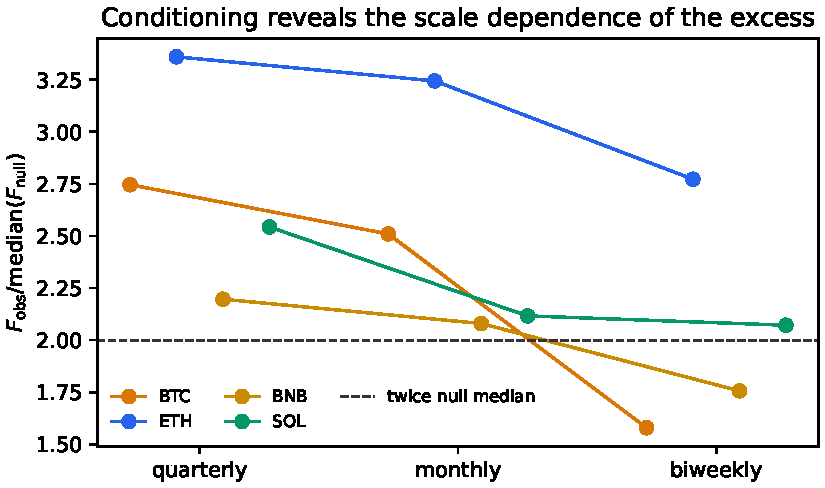
\includegraphics[width=0.85\linewidth]{../output/figuras/fig14_stratification_sensitivity.pdf}
 \caption{Observed weekly raw-flow variance for the primary BTC, ETH, BNB, and
 SOL panel relative to the median of each conditioned null. The dashed line
 marks a factor of two.}
 \label{fig:supp-null}
\end{figure}

\section{Wavelet control of mean drift}

The wavelet estimators are applied directly to the hourly signed-flow series,
not to a separately integrated profile. A Daubechies wavelet with $p$ vanishing
moments annihilates polynomial trends of degree smaller than $p$
\cite{daubechies1992,percival2000}. Thus db1 (Haar) removes a constant mean,
db2 a linear trend, and db3 a quadratic trend.

The implementation is calibrated on fractional Gaussian noise with known
$\nu=1.40$. The block-variance, db1, db2 and db3 estimates agree within $0.01$
without drift. Injecting linear or quadratic trends inflates the block estimate
while leaving the appropriate wavelet estimates fixed. On market data all three
wavelet estimates remain superdiffusive, $\nu=1.10$--$1.36$
[Table~\ref{tab:supp-wavelets}], but their local slopes do not resolve the
monotone crossover seen in the drift-sensitive block variance. This establishes
finite-window superdiffusion while leaving the local crossover undecided.

\section{Scaling model reassessment}

For $C(\tau)\sim\tau^{-a}$, the map $\nu=2-a$ applies only for $0<a<1$.
At $a=1$ the leading form is $T\log T$, and for $a>1$ the generic leading form
is $T$ when the integrated covariance is nonzero; exact cancellation can remove
that term. Applying this map asset by asset gives Table~\ref{tab:supp-scaling}. The single broad-window
power-law model misses all eight block-variance exponents by more than three
reported block-fit standard errors, although those discrepancies do not include
uncertainty in the ACF prediction. The two-regime intervals are weaker still:
they omit amplitudes and crossover uncertainty, and BNB lies outside its band.
We therefore use neither construction as independent confirmation. The exact
finite-sample covariance identity already fixes $V_T$ from $C(\tau)$; the
robust empirical statement is finite-window superdiffusion under drift-resistant
estimators.

Figure~\ref{fig:supp-scaling} shows both constructions. We place them in the
Supplemental Material because they are consistency checks rather than
independent evidence for the finite-window exponent.

\begin{figure}[t]
 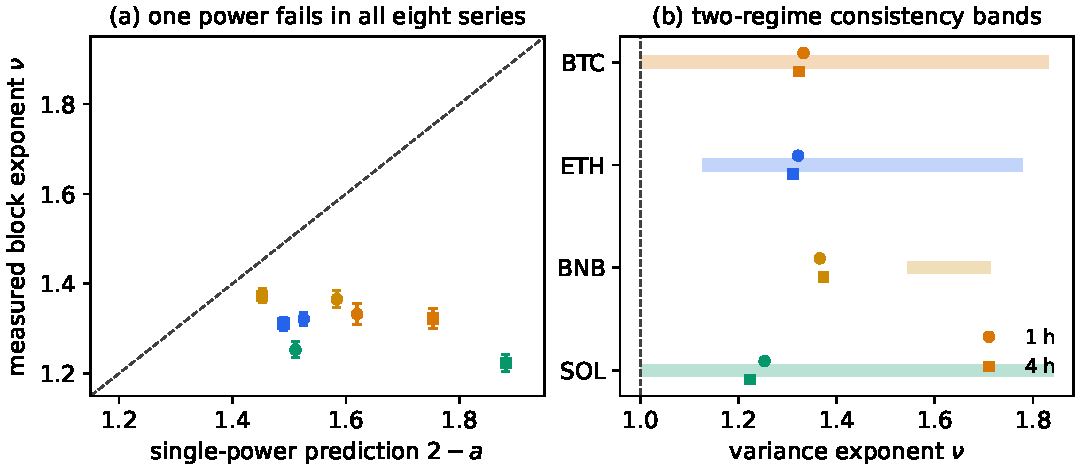
\includegraphics[width=0.92\linewidth]{../output/figuras/fig16_scaling_reassessment.pdf}
 \caption{Scaling reassessment. (a) The broad-window single-power prediction
 misses all eight asset--resolution series; circles and squares denote hourly
 and four-hourly data. (b) Asset-specific two-regime consistency bands, with
 BNB outside its own. Amplitudes and crossover uncertainty are not included, so
 the bands are not quantitative predictions.}
 \label{fig:supp-scaling}
\end{figure}

\section{Calibration of statistical inference}

The main text uses controlled nulls because several standard procedures are
miscalibrated on these heavy-tailed, persistent series. For the
Diebold--Mariano comparison \cite{diebold1995} with Newey--West standard errors
\cite{neweywest1987}, we generated the null distribution by running the
identical analysis after permutation. At a nominal $5\%$ level the empirical
rejection rate is $4$--$6\%$ for BTC but $16$--$18\%$ for ETH, whose null test
statistic has standard deviation about $2.1$ rather than $1.0$. Nominal
$p$ values are therefore not comparable across assets.

Multiplicity creates a second failure mode. A sweep over $144$ combinations
of asset, interval, window, horizon, and baseline contains a cell with nominal
$p=2\times10^{-4}$. Under a Westfall--Young maxT correction
\cite{westfall1993}, however, the maximum null statistic has mean $3.775$, above
the observed maximum $3.667$, and the global value is $p=0.43$. Five cells pass
the uncorrected $5\%$ threshold, fewer than the $7.2$ expected by chance. This
calculation is a calibration result, not evidence of predictability.

Persistent regressors can also produce large out-of-sample correlations with
no information. An independent AR(1) feature reaches correlations $0.21$ for
BTC and $0.32$ for ETH, exceeding the corresponding measured feature. For this
reason, every negative analysis is paired with an injection--recovery control
that carries the tested effect by construction. The positive control verifies
sensitivity; the null then tests whether the real data contain the effect.

The memory estimators were calibrated on exact fractional Gaussian noise
generated by the Davies--Harte circulant method \cite{davies1987}. Over
$\gamma\in[0.4,0.8]$ with $4\times10^5$ samples, the mean absolute errors are
$0.011$ for the wavelet estimate, $0.023$ for detrended fluctuation analysis,
$0.026$ for correlation regression, and $0.068$ for the log-periodogram. On
the market data the four estimates differ by $0.23$--$0.53$, while the wavelet
log-scale diagram rejects a single straight line. Their disagreement is
consistent with scale dependence; the calibration excludes failure on the
tested Gaussian control, not every estimator-specific bias in market data.

\section{Post-shock normalisation and the placebo clock}

Shocks are defined as absolute returns above the $99.5$th percentile, subject
to a minimum temporal separation, and yield $240$ hourly post-event
trajectories. The mean is normalised by the volatility measured immediately
before each event. Excluding the initial fast regime, a power-law fit gives the
amplitude exponent $\beta=0.61\pm1.01$. Six of ten asset--resolution fits reach
an optimiser bound, so the fit does not resolve a nonzero or universal Omori
exponent. Published equity estimates near $0.22$--$0.32$
\cite{lillo2003,zawadowski2006} are quoted only for context.

The same normalisation is applied to the two-time correlation. Its fitted
correlation time grows monotonically across waiting-time bins, but randomly
placed events reproduce the same median Spearman coefficient, $+1.00$. The
pre-event denominator introduces a common slowly varying factor as the process
moves away from its initial scale. Finite-sample autocorrelation bias cannot
separate observation from placebo: the number of trajectories is constant
across waiting-time bins, and the same bias is present in the random-event
ensemble. The comparison therefore supports only the negative statement in
the main text.

\section{Numerical controls for the mesoscopic benchmark}

The benchmark uses a noninteracting level at $\eps_0=0$, temperature $0.05$,
and bias $V=0.3$. The structured hybridisation combines a wide Lorentzian with
coupling $\Gamma=0.5$ and width $4.0$ and a narrow component with coupling
$0.2$ and width $0.04$. The two-time calculation uses $2561$ points with
$\mathrm{d}t=0.125$ over $t\in[-120,200]$ relative to the quench. The
equilibrium relaxation rate differs from the analytic width by $0.33\%$, the
scattering unitarity defect is $8\times10^{-16}$, and independent evaluations
of the zero-frequency noise and second counting cumulant differ by
$1.3\times10^{-9}$.

The device is used only to compare structures. Its conventional Fano factor is
$0.332$--$0.341$, and its finite-window counting exponent is $0.94$--$0.99$.
Neither number is put on the market's transfer-size normalisation. A separate
bias sweep produces a maximum in a fixed-window fitted rate while the exact
pole rates remain smooth. The companion Letter gives the spectral analysis;
the point retained here is methodological: a fitted rate need not identify a
relaxation mode.

\section{Cross-memory diagnostic and a nonidentified candidate}

The exhaustive whole-week shift diagnostic in Sec.~\ref{sec:supp-attribution}
sets the scope of this section. The cross term is not a pure coupling
statistic: even independent sign and magnitude paths retain the product of
their marginal memories in Eq.~\eqref{eq:supp-crossid}. The shifts preserve
those marginal paths and their hour-of-week phase while breaking observed
sign--magnitude pairing. Under the null-aligned reference, the observed cross
term is extreme in all eight series; under the global reference, raw BNB is the
one exception (Table~\ref{tab:supp-weekshift}). Thus the test establishes a
residual relative to this particular preservation rule, not a complementary
causal fraction or a microscopic origin for the residual.

The sample cross correlation changes sign at intermediate lags, but this is not
established as a dynamical reversal. Demeaning within calendar strata imposes a
negative lag-count-weighted sum on a sample covariance and produces an exact
anticorrelation at weekly harmonics. Synthetic series with no population-level
reversal can consequently show crossovers in the observed range after the same
preprocessing. A two-phase episode, in which a same-sign elevated-volume phase
is followed by an opposite-sign unwinding phase, is a minimal construction that
can reproduce a positive short-lag and negative delayed cross correlation. It
is retained only as a candidate: neither the data nor the decomposition
identifies such episodes as the market mechanism.

\section{Phenomenological response-field representation}

This construction is an organisational second-order model, not a microscopic
model of a market. Let $\eps(t)$ be a Gaussian field with mean $\bar\mu$ and
measured covariance kernel $\mathcal K=C_\eps$. A classical doubled-field
representation may be written as
\begin{equation}
 S_\eps=\int\!\dd t\,\tilde\eps(t)[\eps(t)-\bar\mu]
 -\frac12\iint\!\dd t\,\dd t'\,
 \tilde\eps(t)\mathcal K(t-t')\tilde\eps(t').
\end{equation}
It encodes the supplied second-order kernel; it does not derive that kernel or
the origin of order-flow memory. The corresponding counting generating
function is therefore exactly quadratic,
\begin{equation}
 F_T(\chi)=\ln\avg{e^{\chi Q_T}}
 =\chi m_T+\frac12\chi^2V_T,
 \qquad
 V_T=\sum_{t,t'=1}^{T}C_\eps(t-t').
\end{equation}
The variance reconstruction and the linear Gaussian symmetry in the main
analysis are consequently closures of this specified second-order description,
not independent support for it.

For a compact representation of the observed nearly flat lagged response, let
$w_t$ denote the innovation in the Wold decomposition
\begin{equation}
 \eps_t-\bar\mu=\sum_{k\geq0}h_k w_{t-k},\qquad
 \avg{w_t w_s}=\sigma_w^2\delta_{ts}.
\end{equation}
If the price increment couples to $w_t$ rather than to the predictable part of
flow, then $\mathrm{cov}(p_{t+\tau}-p_t,\eps_t)$ is independent of
$\tau\geq1$. This is the familiar surprise mechanism
\cite{gerig2008,jaisson2014,muhlekarbe2026}; here it is a consistency model for
the response convention. The derivative ratio $-C'_\eps/R$ is not interpreted
as a temperature because its uncertainty is unresolved and its shape is largely
fixed once $R$ is nearly flat.

\begin{table}[!htbp]
\caption{Standardised cumulants at the endpoints of the dyadic scale grid. Intervals in Fig.~\ref{fig:supp-cumulants} use the full grid.}
\label{tab:supp-cumulants}
\begin{ruledtabular}
\begin{tabular}{lrrrr}
 & $\gamma_1(1)$ & $\gamma_1(128)$ & $\gamma_2(1)$ & $\gamma_2(128)$ \\
\colrule
BTC & -0.10 & -0.55 & 1.24 & 0.12 \\
ETH & -0.09 & -1.40 & 0.76 & 8.53 \\
BNB & 0.02 & -0.63 & 0.54 & 1.60 \\
SOL & -0.02 & -0.47 & 0.61 & 1.17 \\
\end{tabular}
\end{ruledtabular}
\end{table}

\begin{table*}[!htbp]
\caption{Decomposition of weekly variance amplification under quarterly $\times$ hour-of-week conditioning. $R_J$, $R_S$, and $R_M$ divide observed variance by the median joint-order, sign-order, and magnitude-order null. The interval is an eight-week moving-block bootstrap interval for $R_J$, conditional on its null median.}
\label{tab:supp-decomposition}
\begin{ruledtabular}
\begin{tabular}{llrrrr}
asset & flow & $R_J$ & $R_S$ & $R_M$ & $95\%$ interval for $R_J$ \\
\colrule
BTC & raw & 2.75 & 2.82 & 2.14 & [1.65,4.26] \\
BTC & normalized & 3.20 & 3.35 & 1.64 & [2.32,4.14] \\
ETH & raw & 3.36 & 3.43 & 2.10 & [2.43,4.38] \\
ETH & normalized & 4.22 & 4.43 & 1.89 & [2.90,6.11] \\
BNB & raw & 2.19 & 2.29 & 1.66 & [1.71,2.72] \\
BNB & normalized & 4.20 & 4.39 & 1.86 & [3.05,5.53] \\
SOL & raw & 2.55 & 2.61 & 1.75 & [1.95,3.19] \\
SOL & normalized & 2.99 & 3.14 & 1.52 & [2.22,3.81] \\
\colrule
XRP & raw & 5.67 & 5.81 & 1.81 & [3.10,9.10] \\
XRP & normalized & 5.64 & 5.93 & 1.87 & [4.13,7.33] \\
ADA & raw & 2.08 & 2.10 & 1.75 & [1.50,2.72] \\
ADA & normalized & 2.83 & 2.98 & 1.59 & [1.99,3.83] \\
DOGE & raw & 3.26 & 3.29 & 2.11 & [1.84,5.37] \\
DOGE & normalized & 3.99 & 4.19 & 1.71 & [3.06,4.98] \\
AVAX & raw & 2.36 & 2.53 & 1.57 & [1.56,3.30] \\
AVAX & normalized & 3.18 & 3.35 & 1.55 & [2.40,4.02] \\
\end{tabular}
\end{ruledtabular}
\end{table*}

\begin{table*}[!htbp]
\caption{Exact finite-sample attribution under the primary quarterly $\times$ hour-of-week conditioning. $A=V_{\rm obs}/V_0$, where $V_0$ is the analytic expectation of the joint-order null. Fractions divide the variance excess $V_{\rm obs}-V_0$ into sign order at stratum-homogenised magnitudes and the exact sign--size remainder. Intervals use a paired eight-week circular moving-block bootstrap.}
\label{tab:supp-exact-attribution}
\begin{ruledtabular}
\begin{tabular}{llrrrrr}
asset & flow & $A$ & sign share & coupling share & coupling 95\% interval & $P(f_{sm}>1/2)$ \\
\colrule
BTC & raw & 2.75 & 0.21 & 0.79 & [0.63,0.88] & 1.000 \\
BTC & normalized & 3.16 & 0.46 & 0.54 & [0.45,0.62] & 0.816 \\
ETH & raw & 3.32 & 0.30 & 0.70 & [0.62,0.78] & 1.000 \\
ETH & normalized & 4.24 & 0.41 & 0.59 & [0.49,0.66] & 0.962 \\
BNB & raw & 2.18 & 0.35 & 0.65 & [0.52,0.76] & 0.987 \\
BNB & normalized & 4.18 & 0.41 & 0.59 & [0.53,0.65] & 0.998 \\
SOL & raw & 2.53 & 0.35 & 0.65 & [0.55,0.74] & 0.998 \\
SOL & normalized & 2.96 & 0.51 & 0.49 & [0.35,0.60] & 0.430 \\
\colrule
XRP & raw & 5.64 & 0.48 & 0.52 & [0.43,0.60] & 0.683 \\
XRP & normalized & 5.63 & 0.44 & 0.56 & [0.49,0.63] & 0.956 \\
ADA & raw & 2.06 & 0.27 & 0.73 & [0.60,0.83] & 0.997 \\
ADA & normalized & 2.82 & 0.46 & 0.54 & [0.47,0.64] & 0.867 \\
DOGE & raw & 3.25 & 0.29 & 0.71 & [0.58,0.78] & 1.000 \\
DOGE & normalized & 3.97 & 0.46 & 0.54 & [0.47,0.61] & 0.856 \\
AVAX & raw & 2.34 & 0.44 & 0.56 & [0.40,0.64] & 0.831 \\
AVAX & normalized & 3.16 & 0.51 & 0.49 & [0.41,0.58] & 0.436 \\
\end{tabular}
\end{ruledtabular}
\end{table*}

\begin{table*}[!htbp]
\caption{Conditioning-scale sensitivity of the exact coupling share in the primary panel. Biweekly strata contain at most two observations; after within-stratum demeaning their residual magnitudes are equal, so the coupling component is structurally unidentifiable and reported as degenerate rather than as evidence of absence.}
\label{tab:supp-attribution-sensitivity}
\begin{ruledtabular}
\begin{tabular}{lllrrr}
asset & flow & conditioning & coupling share & 95\% interval & status \\
\colrule
BTC & raw & quarterly & 0.79 & [0.63,0.88] & identified \\
BTC & raw & monthly & 0.47 & [0.40,0.55] & identified \\
BTC & raw & biweekly & 0.00 & [-0.00,0.00] & degenerate \\
BTC & normalized & quarterly & 0.54 & [0.45,0.62] & identified \\
BTC & normalized & monthly & 0.49 & [0.39,0.56] & identified \\
BTC & normalized & biweekly & -0.00 & [-0.00,0.00] & degenerate \\
ETH & raw & quarterly & 0.70 & [0.62,0.78] & identified \\
ETH & raw & monthly & 0.45 & [0.37,0.53] & identified \\
ETH & raw & biweekly & -0.00 & [-0.00,0.00] & degenerate \\
ETH & normalized & quarterly & 0.59 & [0.49,0.66] & identified \\
ETH & normalized & monthly & 0.45 & [0.36,0.51] & identified \\
ETH & normalized & biweekly & 0.00 & [-0.00,0.00] & degenerate \\
BNB & raw & quarterly & 0.65 & [0.52,0.76] & identified \\
BNB & raw & monthly & 0.49 & [0.40,0.66] & identified \\
BNB & raw & biweekly & 0.00 & [-0.00,0.00] & degenerate \\
BNB & normalized & quarterly & 0.59 & [0.53,0.65] & identified \\
BNB & normalized & monthly & 0.45 & [0.37,0.51] & identified \\
BNB & normalized & biweekly & 0.00 & [-0.00,0.00] & degenerate \\
SOL & raw & quarterly & 0.65 & [0.55,0.74] & identified \\
SOL & raw & monthly & 0.49 & [0.39,0.59] & identified \\
SOL & raw & biweekly & 0.00 & [0.00,0.00] & degenerate \\
SOL & normalized & quarterly & 0.49 & [0.35,0.60] & identified \\
SOL & normalized & monthly & 0.41 & [0.31,0.51] & identified \\
SOL & normalized & biweekly & 0.00 & [-0.00,0.00] & degenerate \\
\end{tabular}
\end{ruledtabular}
\end{table*}

\begin{table*}[!htbp]
\footnotesize
\setlength{\tabcolsep}{8pt}
\caption{Sensitivity of the joint weekly variance null. $R_{50}=V_{\rm obs}/\mathrm{median}(V_{\rm null})$ and $R_{98.75}=V_{\rm obs}/Q_{0.9875}(V_{\rm null})$. Primary quarterly rows use 9999 permutations; monthly and biweekly rows use 1999.}
\label{tab:supp-null}
\begin{ruledtabular}
\begin{tabular}{lllrrrr}
asset & flow & conditioning & $R_{50}$ & $R_{98.75}$ & $p_{\rm emp}$ & fixed fraction \\
\colrule
BTC & raw & quarterly & 2.75 & 2.08 & $0.0001$ & 0.00\% \\
BTC & raw & monthly & 2.52 & 1.83 & $0.0005$ & 0.14\% \\
BTC & raw & biweekly & 1.57 & 1.07 & $0.0070$ & 0.97\% \\
BTC & normalized & quarterly & 3.20 & 2.48 & $0.0001$ & 0.00\% \\
BTC & normalized & monthly & 2.67 & 2.05 & $0.0005$ & 0.14\% \\
BTC & normalized & biweekly & 2.27 & 1.59 & $0.0005$ & 0.97\% \\
ETH & raw & quarterly & 3.36 & 2.63 & $0.0001$ & 0.00\% \\
ETH & raw & monthly & 3.23 & 2.41 & $0.0005$ & 0.14\% \\
ETH & raw & biweekly & 2.79 & 1.87 & $0.0005$ & 0.97\% \\
ETH & normalized & quarterly & 4.22 & 3.35 & $0.0001$ & 0.00\% \\
ETH & normalized & monthly & 3.54 & 2.78 & $0.0005$ & 0.14\% \\
ETH & normalized & biweekly & 2.84 & 2.09 & $0.0005$ & 0.97\% \\
BNB & raw & quarterly & 2.19 & 1.69 & $0.0001$ & 0.00\% \\
BNB & raw & monthly & 2.07 & 1.54 & $0.0005$ & 0.14\% \\
BNB & raw & biweekly & 1.75 & 1.17 & $0.0015$ & 0.97\% \\
BNB & normalized & quarterly & 4.20 & 3.29 & $0.0001$ & 0.00\% \\
BNB & normalized & monthly & 3.59 & 2.81 & $0.0005$ & 0.14\% \\
BNB & normalized & biweekly & 3.35 & 2.44 & $0.0005$ & 0.97\% \\
SOL & raw & quarterly & 2.55 & 2.02 & $0.0001$ & 0.00\% \\
SOL & raw & monthly & 2.12 & 1.63 & $0.0005$ & 0.14\% \\
SOL & raw & biweekly & 2.10 & 1.45 & $0.0005$ & 0.97\% \\
SOL & normalized & quarterly & 2.99 & 2.36 & $0.0001$ & 0.00\% \\
SOL & normalized & monthly & 2.20 & 1.73 & $0.0005$ & 0.14\% \\
SOL & normalized & biweekly & 2.31 & 1.68 & $0.0005$ & 0.97\% \\
\end{tabular}
\end{ruledtabular}
\end{table*}

\begin{table}[!htbp]
\caption{Global exponent $\nu$ over $T=8,\ldots,256$. db1 removes a constant, db2 a linear trend, and db3 a quadratic trend.}
\label{tab:supp-wavelets}
\begin{ruledtabular}
\begin{tabular}{lrrrr}
asset & block variance & db1 & db2 & db3 \\
\colrule
BTC & 1.42 & 1.20 & 1.14 & 1.13 \\
ETH & 1.37 & 1.24 & 1.26 & 1.29 \\
BNB & 1.43 & 1.35 & 1.36 & 1.30 \\
SOL & 1.31 & 1.15 & 1.13 & 1.10 \\
\end{tabular}
\end{ruledtabular}
\end{table}

\FloatBarrier
\refstepcounter{table}
\label{tab:supp-scaling}
\noindent\textsc{Table \thetable.} Asset-specific scaling reassessment. The consistency band maps $C(\tau)\sim\tau^{-a}$ to $\nu=2-a$ only for $a<1$; $a>1$ maps to diffusion. Amplitudes are not fitted, so the band is not a quantitative prediction.
\begin{center}
\begin{ruledtabular}
\begin{tabular}{lrrrrr}
asset & $a_f$ & $a_s$ & consistency band & $\nu_{1h}$ & $\nu_{4h}$ \\
\colrule
BTC & 1.00 & 0.17 & [1.00,1.83] & 1.33 & 1.32 \\
ETH & 0.87 & 0.22 & [1.13,1.78] & 1.32 & 1.31 \\
BNB & 0.46 & 0.29 & [1.54,1.71] & 1.37 & 1.37 \\
SOL & 1.71 & 0.16 & [1.00,1.84] & 1.25 & 1.22 \\
\end{tabular}
\end{ruledtabular}
\end{center}

\FloatBarrier

\bibliographystyle{apsrev4-2}
\bibliography{refs}

\end{document}
